\documentclass[12pt, a4paper]{article}

\usepackage[utf8]{inputenc}
\usepackage[portuguese]{babel}
\usepackage{amsmath}
\usepackage[T1]{fontenc}
\usepackage{amssymb}
\usepackage{indentfirst}
\usepackage{subfigure}
\usepackage[version=4]{mhchem}
\usepackage[font=small,labelfont=bf]{caption}

\usepackage[nottoc]{tocbibind}

\usepackage{geometry}
 \geometry{a4paper,
 left=3cm,
 top=3cm,
 bottom=3cm,
 right=3cm
 }

\usepackage{graphicx}
\graphicspath{ {./figures/} }

	\title{
{Transições de Fase no Modelo de Ising 2D}\\
{\large Modelação e Física Estatística}\\ \vspace{3cm}
{
\includegraphics[scale=0.5]{Logo_UA.png}}
\vspace{6cm}
}
	\author{Alexandre Rodrigues (92993) \\
	João Inácio	(93039)}
	\date{\today}

\begin{document}
	\maketitle 
		
	\newpage
	
	\section{Modelo de Ising}
	
	No ano de 1920 Wilhelm Lenz, um físico alemão, deu a Ernest Ising, seu estudante de doutoramento, um exercício em que era considerado uma cadeia uni-dimensional de partículas de spin-1/2 que podiam estar a apontar para cima ou para baixo. Os spins interagiam apenas com os seus vizinhos mais próximos. Cinco anos mais tarde, Ising consegui resolver o modelo, sendo premiado com um doutoramento em física. Este concluiu que a uma dimensão não havia transição de fase e, incorretamente, extrapolou que para dimensões maiores, também não havia transições de fase. Mais tarde, em 1944, um físico americano Lars Onsager resolveu analiticamente o mesmo modelo, mas a duas dimensões. Com isto provou que havia uma transição de fase, de um estado ordenado a baixas temperaturas, onde os spins das partículas alinhavam-se segundo o mesmo eixo, para um estado desordenado a altas temperaturas, onde configurações com spins vizinhos anti paralelos eram favorecidas. Ainda não há uma solução analítica para três u mias dimensões,só conseguimos obter estimativas através de métodos numéricos. Desde então o modelo de Ising é um dos modelos físicos mais publicado e estudo devido à sua simplicidade e transição de fase não trivial.
	
	Este modelo pode representar um material ferromagnético, onde a baixas temperaturas exibe uma magnetização espontânea e a uma certa temperatura, a temperatura de Curie $T_C$, ocorre uma transição de fase para um estado paramagnético. Metais de transição, Ferro, Níquel, Cobalto, e alguns metais raros, como o Gadolínio, exibem este tipo de comportamento.
	
	Como o modelo de Ising representa um sistema de partículas de spin-1/2, que podem estar a apontar para cima $(+1)$ ou para baixo $(-1)$, onde só há interação entre partículas vizinhas, o seu Hamiltoniano é escrito 
\begin{equation}
	\mathcal{H} = -\sum_{<i,j>} J_{ij} S_i S_j - H \sum_iS_i,
\end{equation}
onde $J$ é a constante de interação entre spins vizinhos, $S_i$ o valor do spin da partícula no local $i$ e $H$ é um campo magnético externo aplicado. A notação $<i,j>$ do somatório significa que a soma é efetuada sobre os vizinhos da partícula $i$. Se $J>0$, o sistema a temperaturas baixas comporta-se como de uma maneira ferromagnetica e se $J<0$ comporta-se como um sistema paramagnético.

	Neste trabalho, não vamos estudar o modelo de Ising com um campo magnético aplicado, por isso $H=0$, e vamos considerar que a constante de interação é igual à unidade, $J=1$. Assim o hamiltoniano fica
\begin{equation}
	\mathcal{H} = -\sum_{<i,j>} S_i S_j \equiv -\frac{1}{2} \sum_{ij} S_i S_j.
\end{equation}

	\pagebreak

	\subsection{Densidade de Estados Conjunta}

	A densidade de estados $g(E)dE$ é definida como o número de microestados disponíveis ao sistema num intervalo de energia de $E$ a $E + dE$. Para um sistema discreto, a densidade de estados $g(E)$ dá-nos o número exato de microestados com energia $E$.Com a densidade de estados conseguimos tirar a função partição canónica, $Z(T)$ e a energia livre de Helmholtz, $F(T)$, em função da temperatura.
	
	Como estamos a avaliar um sistema magnético, é-nos útil saber quantos microestados o sistema tem disponível por energias e magnetizações. Assim, usamos a densidade de estados conjunta, um histograma a duas dimensões que contém informação sobre o número de microestados com uma dada energia $E$ e magnetização $M$, $g(E, M)$. Com a densidade de estados conjunta, conseguimos obter a função partição canónica e a energia livre ambas em função da temperatura e magnetização do sistema.
	
	Para um sistema Ising a duas dimensões numa rede quadrada de lado $L=2$, a densidade de estados conjunta fica
	\begin{table}[h]
	\centering
	\caption{Densidade de estados conjunta para um sistema Ising 2D numa rede quadrada de lado $L=2$. As colunas representam as magnetizações $M$ e as linhas as energias $E$ disponíveis.}
	\label{exact_L2}
	\begin{tabular}{l|lllll}
	$E \ / \ M$ & $-4$ & $-2$ &  $0$ & $+2$ &  $+4$ \\ \hline
	$-8$  & 1  & 0  & 0 & 0 & 1 \\
	$-4$  & 0  & 0  & 0 & 0 & 0 \\
	$0$   & 0  & 4  & 4 & 4 & 0 \\
	$+4$   & 0  & 0  & 0 & 0 & 0 \\
	$+8$   & 0  & 0  & 2 & 0 & 0
	\end{tabular}
	\end{table}
	
	\begin{figure}[h]
	\centering
	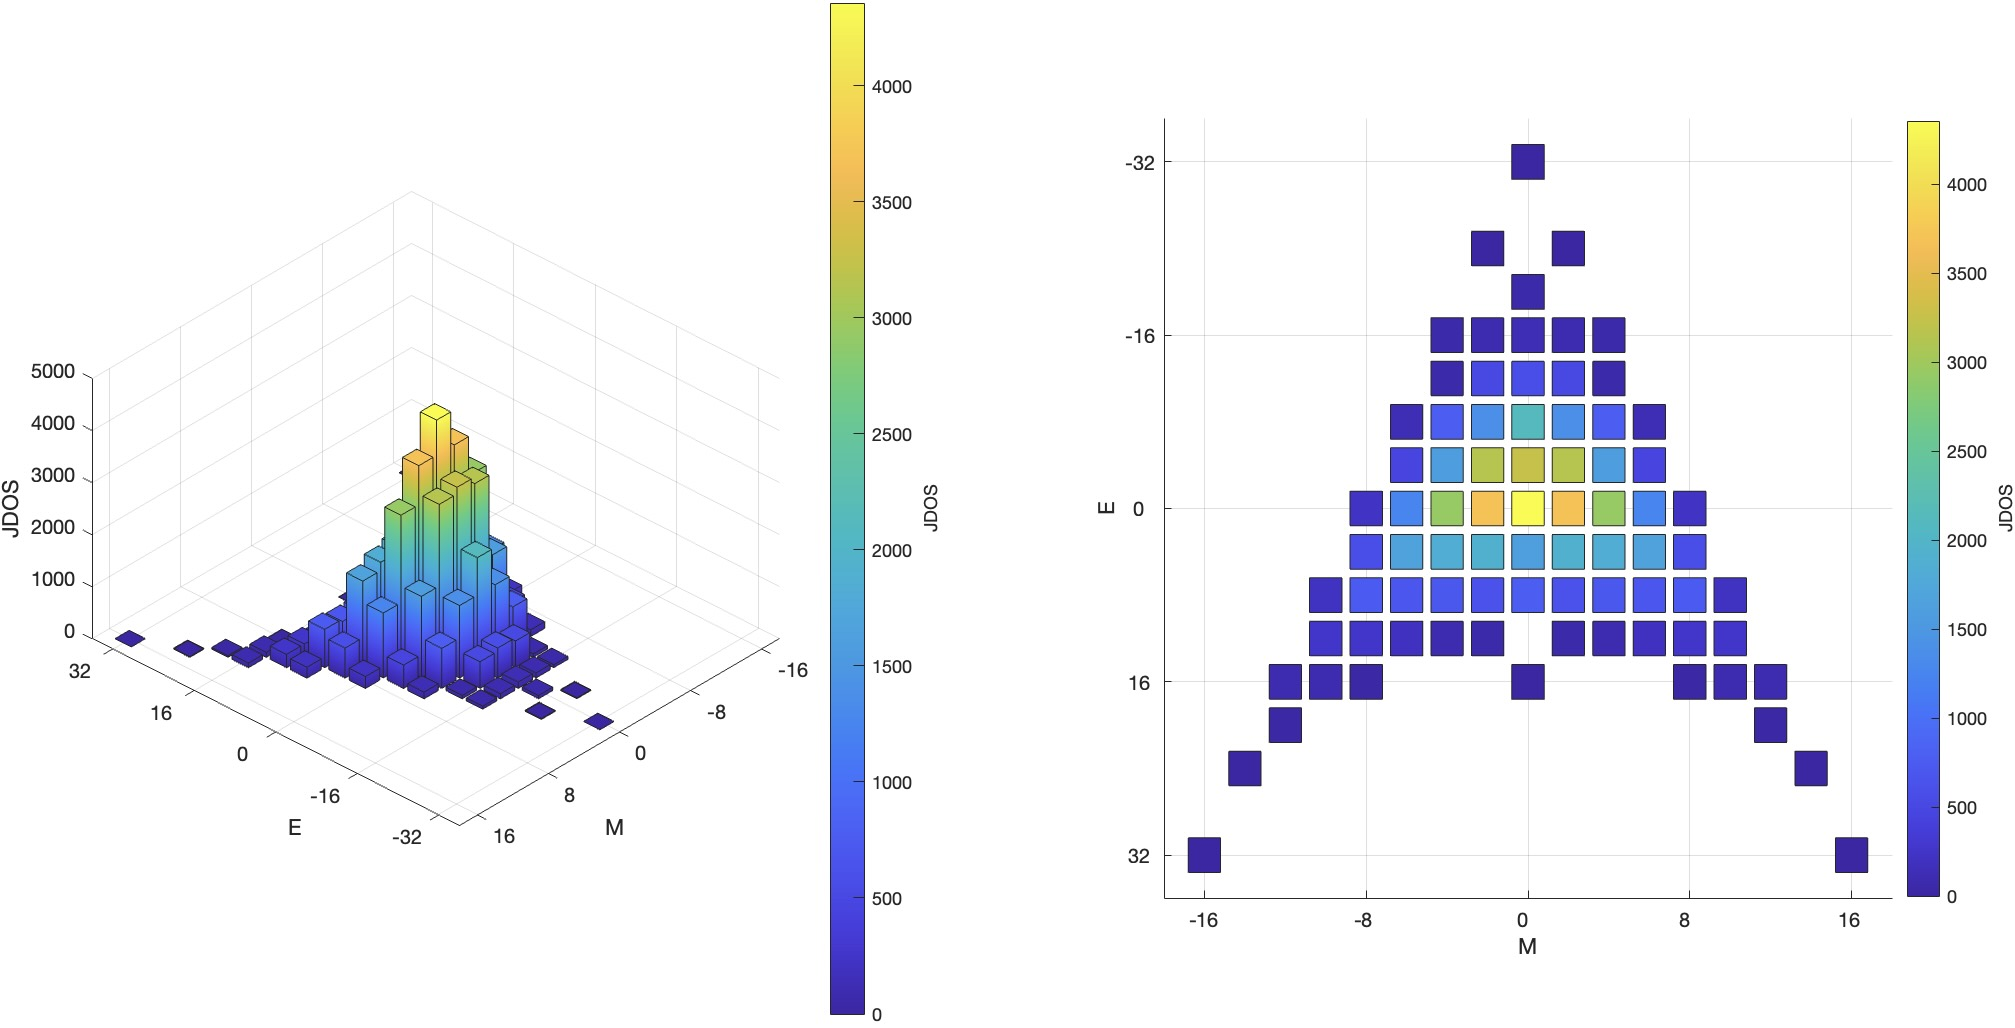
\includegraphics[scale=0.20, height=4.5cm]{JDOS_exact_L4_SS.jpeg}
	\caption{Gráfico da densidade de estados conjunta exata para um sistema Ising 2D numa rede quadrada de lado $L=4$. }
	\label{exact_L4}
	\end{figure}
	
	Para obter estes  resultados, tivemos de visitar todas os microestados do espaço de fases $(E, M)$, disponíveis ao sistema. Para sistemas pequenos (até $L=4$ numa rede a duas dimensões) isto é fazível, contudo para sistemas maiores, onde o número de configurações fica  muito elevado, este processo fica muito demorado e é ineficiente. Por exemplo uma rede quadrada com lado $L=8$ tem $2^{256} \approx	 1E77$ configurações e já é impossível determinar a densidade de estados através deste método. Na secção 2, iremos apresentar um método eficiente para tal.
	
		\subsection{Relações Termodinâmicas}

	Tendo a densidade de estados conjunta, conseguimos obter quais quer variáveis termodinâmicas num sistema em equilíbrio. 
	A probabilidade de um estado com energia $E_i$, é dada por
\begin{equation}
	P_i = \frac{\sum_q g(E_i, M_q) \exp(-\beta E_i)}{Z},
\end{equation}
onde $\beta$ é definido como $\beta \equiv 1/k_BT$ e $Z$ é a função partição canónica, 
\begin{equation}
	Z = \sum_q Z(T, M_q) = \sum_q \sum_i g(E_i, M_q) \exp(-\beta E_i).
\end{equation}
Com isto conseguimos obter médias de ensemble, 
\begin{equation}
	\langle E \rangle = \frac{1}{Z} \sum_i \sum_q  g(E_i, M_q) E_i \exp(-\beta E_i),
\end{equation}
\begin{equation}
	\langle M \rangle  = \frac{1}{Z} \sum_q \sum_i M_q g(E_i, M_q) \exp(-\beta E_i) \equiv \frac{1}{Z} \sum_q M_q Z(T, M_q).
\end{equation}
$\langle E \rangle$ está relacionado com a capacidade calorifica e $\langle M \rangle$ está relacionado com a suscetibilidade magnética por 
\begin{equation}
	\langle C \rangle = \frac{\langle E^2 \rangle - \langle E \rangle^2}{\left( k_BT \right)^2}, \quad \quad \quad 
	\langle \chi \rangle = \frac{\langle M^2 \rangle - \langle M \rangle^2}{\left( k_BT \right)^2},
\end{equation}
e usando a segunda lei da termodinâmica conseguimos tirar a entropia.
\begin{equation}
	\langle S \rangle= \int \frac{\langle C \rangle}{T} dT.
\end{equation}

	Contudo há uma outra maneira de obter propriedades termodinâmicas, de uma densidade de estados conjunta. Usando a energia livre de Helmholtz, definida por 
\begin{equation}
	F(T, M) = - k_B ln(Z(T, M)) \equiv U - TS
\end{equation}
e o principio de minimização de energia, conseguimos obter $F_{min} (T) = \min(F(M, T))$, que é definido como a menor energia livre dependente da temperatura que pode ser alcançada pelo sistema.Com isto conseguimos obter $M_{F_{min}}$, $E_{F_{min}}$ e as seguintes variáveis
\begin{equation}
	C = - T \frac{\partial^2 F_{min}}{\partial T^2},
\end{equation}

\begin{equation}
	S = - \frac{\partial F_{min}}{\partial T}.
\end{equation}

\pagebreak
	
	\section{Método de Wang-Landau}
	
	Em 2001, Fugao Wang e David P. Landau propuseram um novo método de Monte-Carlo, chamado método de Wang-Landau (WL). O objetivo deste método é tentar estimar a função de partição canónica 
\begin{equation}
	Z = \sum_E g(E) \exp(-\beta E),
\end{equation}
através da estimação da densidade de estados $g(E)$ via uma random walk, com probabilidade proporcional ao inverso da densidade de estados $\frac{1}{g(E)}$, que produz um histograma plano no espaço de energia. A estimativa de $g(E)$ é melhorada a cada iteração do método.
Este método pode ser usado para estimar a densidade de estados conjunta, realizando uma random walk no espaço de fases $(E, M)$ ao invés do espaço de energias. 

Primeiro começamos num ponto aleatório do espaço de fases, $(E_i, M_i)$,  e com uma estimativa da densidade de estados, normalmente $g(E, M)=1$. Começamos a random walk, efetuando um spin-flip que leva o sistema do estado $(E_i, M_i)$ ao estado $(E_j, M_j)$ e aceitamos esta modificação com uma probabilidade
\begin{equation}
	P((E_i, M_i) \rightarrow (E_j, M_j)) = \min\left(1, \frac{g(E_i, M_i)}{g(E_j, M_j)}\right).
\end{equation}
Quer a nova configuração seja aceite ou rejeitada, estamos no ponto $(E, M)$ do espaço de fases e atualizamos o histograma e a densidade de estados segundo,
\begin{equation*}
	H(E, M) = H(E,M)+1, \quad \quad \quad \quad g(E,M)=f \times g(E,M).
\end{equation*}
Aqui, o parâmetro $f$ e chamado de fator de modificação. Uma escolha razoável para este parâmetro no inicio da simulação é $f_0=e$. Se este é demasiado grande vai induzir erros estatísticos na nossa estimativa, caso seja demasiado pequeno a simulação vai ficar muito demorada. 
Este processo é repetido até obtermos um histograma "plano". Como é impossível obter um histograma $100\%$ plano, definimos um critério para a planicidade do histograma como $\min(H(E, M)) > \langle H(E, M) \rangle \times p$. $p$ é escolhido de acordo com o sistema que estamos a simular. Para sistemas pequenos, $p$ pode ser tão grande como $0.95$, contudo para sistemas maiores a condição de planicidade pode nunca ser satisfeita se $p$ for perto da unidade.

Quando o histograma fica plano, fazemos $H(E, M) = 0$ e reduzimos o fator de modificação $\sqrt{f_{i}} \rightarrow f_{i+1}$, de forma a obter uma melhor estimativa da densidade de estados conjunta a cada iteração da simulação. Repetimos isto até que o valor de $f$ seja menor que um dado $f_{final}$, que normalmente define-se como $f_{final}  \sim 1+1E-8$.

No final da simulação temos que normalizar a densidade de estados. Para tal, podemos usar o facto de 
\begin{equation}
	\sum_{EM} g(E,M) = 2^N,
\end{equation}
onde $N$ é o número de partículas no sistema.


	
	\section{Resultados}
	
	
	\section{Conclusão}
	
	\newpage
	\bibliography{citacoes}	
	\bibliographystyle{ieeetr}
	
\end{document}

